\documentclass[a4paper, 12pt]{article}

\usepackage[margin=2cm,lmargin=4cm]{geometry}
\usepackage{parskip, indentfirst}
\def\defparskip{0.5cm}
\def\defparindent{0.5cm}
\parskip=\defparskip
\parindent=\defparskip

\usepackage{newtxtext, newtxmath}

\usepackage{hyperref}
\usepackage{titlesec, titletoc, chngcntr}
\titleformat{\section}[hang]{\center\bfseries\MakeUppercase}{CHAPTER \thesection: }{0pt}{}
\titleformat*{\subsection}{\bfseries}
\titleformat*{\subsubsection}{\bfseries}

\titlecontents{figure}[0pt]{}{Figure \thecontentslabel: }{}{\titlerule*[9pt]{.}\contentspage}
\titlecontents{table}[0pt]{}{Table \thecontentslabel: }{}{\titlerule*[9pt]{.}\contentspage}
\counterwithin{figure}{section}
\counterwithin{table}{section}

\usepackage{graphicx, setspace, multicol, booktabs, array, tikz, fancyhdr}
\usepackage{caption, subcaption, float, enumitem, blindtext}
\usepackage{amsmath, physics, siunitx, flowchart}
\usepackage[]{apacite}

\fancyhead{}
\fancyfoot{}
\fancyfoot[R]{\fontsize{10pt}{10pt}\selectfont\thepage\normalsize}
\renewcommand{\headrulewidth}{0pt}

\setlist{parsep=0pt}
\sisetup{separate-uncertainty=true}
\setkeys{Gin}{width=\linewidth,height=0.2\textheight,keepaspectratio}
\captionsetup{width=0.8\textwidth} %, font=bf}
\usetikzlibrary{arrows.meta}
\numberwithin{equation}{section}

% distance between floats
\setlength{\textfloatsep}{1cm plus 1.0pt minus 1.0pt}
\setlength{\intextsep}{1cm plus 1.0pt minus 1.0pt}
\setlength{\floatsep}{1cm plus 1.0pt minus 1.0pt}

\gdef\date{\today}
\gdef\title{ESTIMATING NEUTRINO FLUX FROM LOW MASS STELLAR MODEL USING MACHINE LEARNING TECHNIQUE}
\gdef\titleMS{MENGANGGARKAN FLUKS NEUTRINO DARIPADA MODEL BINTANG JISIM RENDAH MENGGUNAKAN TEKNIK PEMBELAJARAN MESIN}
\gdef\author{IRFAN MUQRI BIN ABD RAHMAN}
\gdef\matricno{U2103688}
\gdef\IC{(021214-01-0451)}

\begin{document}
\startcontents[default]

\pagestyle{empty}
\titlecontents{section}[0pt]{}{}{}{\titlerule*[9pt]{.}\contentspage}
\newgeometry{hmargin=4cm, vmargin=5cm}

\sffamily\bfseries
\fontsize{16pt}{16pt}\selectfont
\begin{center}
	\title
	\vfill
	\author
	\vfill
	FACULTY OF SCIENCE\\
	UNIVERSITI MALAYA\\
	KUALA LUMPUR

	2024
\end{center}

\clearpage

\rmfamily
\fontsize{14pt}{14pt}\selectfont
\begin{center}
	\title
	\vfill
	\author
	\vfill

	FINAL YEAR PROJECT REPORT SUBMITTED IN PARTIAL FULFILMENT OF THE REQUIREMENTS
	FOR THE DEGREE OF BACHELOR OF SCIENCE IN PHYSICS
	\vspace{2cm}

	DEPARTMENT OF PHYSICS\\
	FACULTY OF SCIENCE\\
	UNIVERSITI MALAYA\\
	KUALA LUMPUR

	2024
\end{center}

\normalfont
\clearpage
\normalsize
\restoregeometry

\pagestyle{fancy}
\pagenumbering{roman}
\setcounter{page}{2}
\parindent=0pt
\parskip=6pt

\begin{center}
	{\bfseries
		UNIVERSITI MALAYA

		ORIGINAL LITERARY WORK DECLARATION
	}
	\vspace{1cm}

\end{center}

Name of Candidate: \author\hfill\IC

Matric No: \matricno

Name of Degree: BACHELOR OF SCIENCE IN PHYSICS

Title of Project Paper (``this Work''):

\title

Field of Study: Experimental Physics
\vspace{1em}

I do solemnly and sincerely declare that:
\begin{enumerate}[label=(\arabic*)]
	\item I am the sole author of this Work;
	\item This Work is original;
	\item Any use of any work in which copyright exists was done by way of fair
	      dealing and for permitted purposes and any excerpt or extract from, or
	      reference to or reproduction of any copyright work has been disclosed expressly
	      and sufficiently and the title of the Work and its authorship have been
	      acknowledged in this Work;

	\item I do not have any actual knowledge nor do I ought reasonably to know that
	      the making of this work constitutes an infringement of any copyright work;

	\item I hereby assign all and every rights in the copyright to this Work to the
	      University of Malaya (``UM''), who henceforth shall be owner of the copyright in
	      this Work and that any reproduction or use in any form or by any means
	      whatsoever is prohibited without the written consent of UM having been first
	      had and obtained;

	\item I am fully aware that if in the course of making this Work I have infringed
	      any copyright whether intentionally or otherwise, I may be subject to legal
	      action or any other action as may be determined by UM.
\end{enumerate}
\vfill

\hspace{1cm}Candidate's Signature\hfill Date:\ \date
\vspace{.1in}

Subscribed and solemnly declared before,
\vfill

\hspace{1cm}Witness's Signature\hfill Date:\ \date

Name:

Designation:

\clearpage
\parskip=\defparskip
\parindent=\defparskip

\doublespacing
\phantomsection
\addcontentsline{toc}{section}{Abstract}

\begin{center}
	\bfseries
	\begin{singlespace}
		\title
	\end{singlespace}

	ABSTRACT
\end{center}

\blindtext[1]

\clearpage
\phantomsection
\addcontentsline{toc}{section}{Abstrak}

\begin{center}
	\bfseries
	\begin{singlespace}
		\titleMS
	\end{singlespace}

	ABSTRAK
\end{center}

\blindtext[1]

\clearpage
\onehalfspacing

\phantomsection
\addcontentsline{toc}{section}{Acknowledgements}

\begin{center}
	\bfseries
	ACKNOWLEDGEMENTS
\end{center}

\blindtext[1]

\clearpage


\parskip=0pt
\parindent=0pt
\doublespacing

\renewcommand{\contentsname}{Table of Contents}
\phantomsection
\section*{\contentsname}
\addcontentsline{toc}{section}{\contentsname}
\printcontents[default]{l}{0}{\setcounter{tocdepth}{2}}
\clearpage

\phantomsection
\addcontentsline{toc}{section}{\listfigurename}
\listoffigures
\clearpage

\phantomsection
\addcontentsline{toc}{section}{\listtablename}
\listoftables
\clearpage

\phantomsection
\xdef\listsymbolname{List of Symbols and Abbreviations}
\section*{\listsymbolname}
\addcontentsline{toc}{section}{\listsymbolname}
\begin{tabular}{l>{:\hspace{0.5cm}}l}
	EA & Example Abbreviation
\end{tabular}
\clearpage

\phantomsection
\xdef\listappendixname{List of Appendices}
\section*{\listappendixname}
\addcontentsline{toc}{section}{\listappendixname}
\startcontents[appendix]
\printcontents[appendix]{l}{0}{\setcounter{tocdepth}{2}}
\stopcontents[appendix]
\clearpage

\parskip=1cm
\parindent=0.5cm

\onehalfspacing
\parindent=0.5cm
\parskip=0.5cm
\pagenumbering{arabic}
\titlecontents{section}[0pt]{\vspace*{1cm}}{\bfseries CHAPTER \thecontentslabel: \uppercase}{}{\titlerule*[9pt]{ }\contentspage}

\section{Introduction}

This is introduction \shortcite{example2002}.

\subsection{Problem Statement}
Neutrinos are present in huge quantities owing to various astrophysical phenomena such as those in a stellar medium like the Sun. Although solar neutrino flux is able to be measured on the Earth by using a detector like Super Kamiokande, neutrinos emitted from distant stars and the physics of their detection still presents a problem because of the difficulty in interaction and the detection of such distant and sparse interactions by current technology. There is no proper means of detecting neutrino radiation from stellar sources at the present time, though theorists continue to make predictions based on elaborate computations.
 
To address these issues, machine learning approaches, which are particularly efficient when it comes to complex data processing tasks and prediction problems located in various physics, would be one of the available options. This study aims to solve the problem by estimating the neutrino flux from a low mass stellar model through the use of a machine learning approach. Here we will try to construct and train a supervised machine learning model aimed at predicting neutrino flux from stars which are not accessible by direct observation, utilizing available solar neutrino flux data and theoretical models.


\subsection{Research Questions}

The research aims to answer the following questions:
\begin{enumerate}
	\item What is the neutrino flux production beyond the Standard Solar Model in low mass stars?
	\item Is machine learning able to give the best estimate in the current solar neutrino productions and what is the limit when extended to beyond the Standard Solar Model? 
	
\end{enumerate}

\subsection{Research Objectives}

The research aims to achieve the following objectives:
\begin{enumerate}
	\item Example.
\end{enumerate}

\subsection{Relevance of Research}

Example.

\clearpage
\section{Literature Review}

\subsection{Subtopics}

Example.

\begin{figure}[H]
  \centering
  
\includegraphics{assets/example.png}
  \caption{Example figure.}
  \label{fig:example}
\end{figure}

Refer to Figure~\ref{fig:example}.

\clearpage
\section{Methodology}

\subsection{Data}

\begin{equation}
    \frac{dL_\nu}{dM_{r}}=\epsilon_{\nu}(\rho,T)
\end{equation}

\begin{equation}
    \mathrm{Flux}=\frac{L}{4\pi r^2}
\end{equation}


\subsection{Machine Learning}
Sci Kit Learn was used, specifically the Linear Regression module:
\begin{equation}
    y=\beta_{0}x_0+\beta_{1}x_1+\beta_{2}x_2+\beta_{3}x_3+...+\beta_{n}x_n
\end{equation}
where 
$y$ is the independent variables, $\beta_0, \beta_{1}, \beta_{2}, \beta_{3},..., \beta_{n}$ is the coefficient. 

The basis of linear regression is the same as $y= mx+c$ but sklearn used more coefficients to predict the model. Linear regression estimate  coefficient such that the sum of error is very small ~  $10^{-4}$ (the tolerance adopted by sklearn). This method is also known as the least square method.

In this project the code will calculate the gradient B (written as J)  between the inputs which are the Masses and the Luminosity and the star ages.
\begin{equation}
    \mqty[
        m_{1}\\m_{2}\\m_{3}  
    ]
    J
    =
    \mqty[
        L_{11}&A_{11}&L_{12}&A_{12}&L_{13}&A_{13}\\
        L_{21}&A_{21}&L_{22}&A_{22}&L_{23}&A_{23}\\
        L_{31}&A_{31}&L_{32}&A_{32}&L_{33}&A_{33}
    ]
    \label{Eq:matrices}
\end{equation}
where $m$ is mass, $L$ is luminosity and $A$ is star age.
Equation\ref{Eq:matrices} is the representation on how the data was arranged in order to do the linear regression method. 

\begin{figure}[H]
    \centering

    \begin{tikzpicture}
        \node (A) at (-4,0) [draw, terminal] {Masses X($n\times 1$ )}; 
        \node (B) at (4,0) [draw, terminal] {Luminosity and Star Age Y($n \times m$)}; 
        \node (C) at (0,-2) [draw, process] {Zeroes Matrix J ($1\times m$)};
        \node (D) at (0,-4) [draw, process] {$\min_{J}||XJ-Y||^{2}$};
        \node (E) at (0,-6) [draw, process] {$J=(X^{T}X)^{-1}X^{T}Y$};
        \node (F) at (0,-8) [draw, process] {$X'J=Y'$};
        \node (G) at (0,-10) [draw, terminal] {OUTPUT};
        \draw[-{Latex}] (A) |- (C);
        \draw[-{Latex}] (B) |- (C);
        \draw[-{Latex}] (C) -- (D);
        \draw[-{Latex}] (D) -- (E);
        \draw[-{Latex}] (E) -- (F);
        \draw[-{Latex}] (F) -- (G);

    \end{tikzpicture}
    \caption{Flowchart of how the code does the linear regression.}
    \label{fig:flow}
\end{figure}

Figure\ref{fig:flow} shows the flow of how the code does the linear regression. The code will take input Masses in the form of X$(n\times1)$ matrix and Luminosity and Star Age as Y$(n\times m)$ matrix. The code will then generate a zeros matrix J$(1\times m)$. The J will then be calculated using Equation\ref{Eq:leastsq} and then used in prediction.

\begin{equation}
    e=\sqrt{(x_p-x_g)^2+(y_p-y_g)^2}
    \label{Eq:er}
\end{equation}

Then using the Equation~\ref{Eq:er}, the error was calculated in term of the offset between predicted and grid data per mass.
\clearpage
\section{Results and Discussion}

\begin{figure}[H]
	\centering
	\begin{subfigure}{\textwidth}
		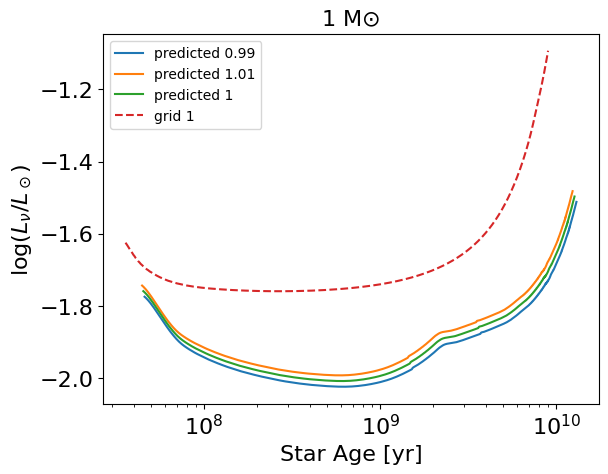
\includegraphics[width=\textwidth,height=0.5\textheight]{assets/output1singlemodel.png}
		\caption{Sun $1M\odot$ Single Testing Data.}
		\label{fig:SunTesta}	
	\end{subfigure}
	\begin{subfigure}{\textwidth}
		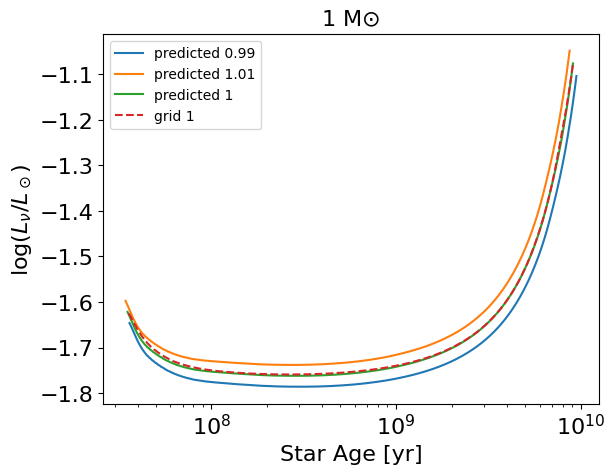
\includegraphics[width=\textwidth,height=0.5\textheight]{assets/output1.png}
		\caption{Sun $1M\odot$ Multi Model($0.5-1.1M_\odot$) Testing Data.}
		\label{fig:SunTestb}	
	\end{subfigure}
	\label{fig:SunTest}
\end{figure}

\begin{figure}[H]
	\centering
	\begin{subfigure}{\textwidth}
		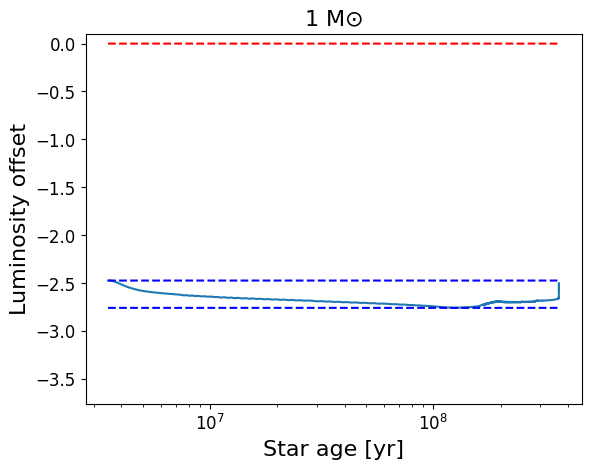
\includegraphics[width=\textwidth,height=0.5\textheight]{assets/error1modelsingle.png}
		\caption{Luminosity Offset for $1M\odot$.}
	\end{subfigure}
	\begin{subfigure}{\textwidth}
		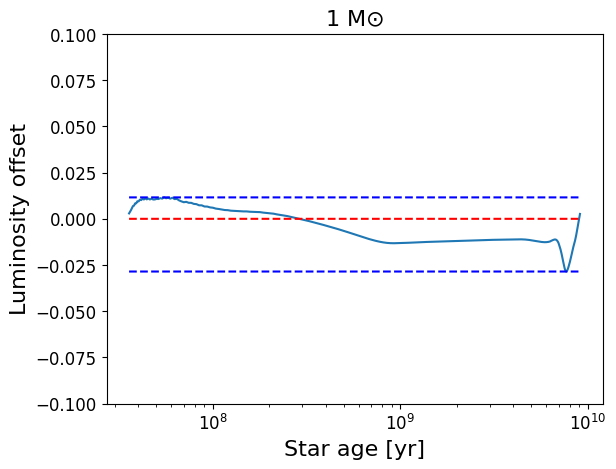
\includegraphics[width=\textwidth,height=0.5\textheight]{assets/error 1.png}
		\caption{Single Multimodel Error.}	
\end{subfigure}
	\label{fig:lumoff}
\end{figure}

\begin{figure}[H]
	\centering
	\begin{subfigure}{\textwidth}
		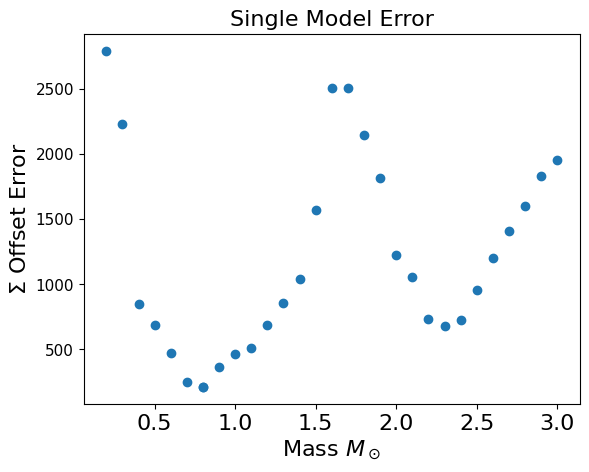
\includegraphics[width=\textwidth,height=0.5\textheight]{assets/singlemodeerror.png}
		\caption{Single Model Error.}
	\end{subfigure}
	\begin{subfigure}{\textwidth}
		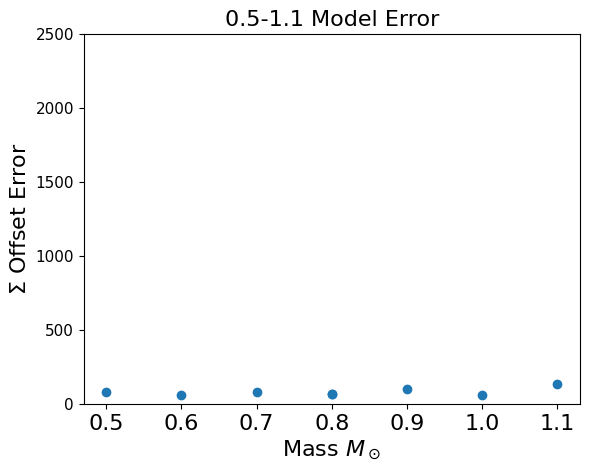
\includegraphics[width=\textwidth,height=0.5\textheight]{assets/0.5-1.1Error.png}
		\caption{$0.5-1.1M\odot$ Model Error.}
	\end{subfigure}
	\label{fig:sumerror}
\end{figure}

\begin{table}[H]
    \centering
	\caption{Stars with their mass and distance.}
	\label{tab:stars and mass}
	\begin{tabular}{ccc}
		\toprule
		Star & Mass [$M\odot$]  & Distance [$pc$] \\
		\midrule
		$\tau$ ceti & $0.78$ & $3.65$\\
		Sun & $1$ & $4.85\times 10^{-6}$\\
		 & $1$ & $4.85\times 10^{-6}$\\
		\bottomrule
	\end{tabular}
\end{table}

\begin{figure}[H]
	\centering
	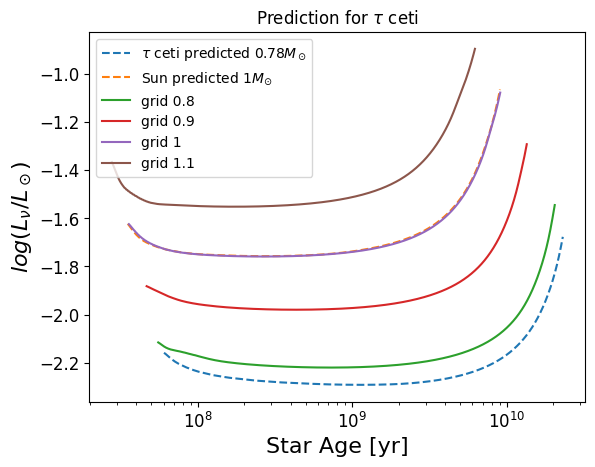
\includegraphics[width=\textwidth,height=0.5\textheight]{assets/predtauceti.png}
	\caption{Prediction for $\tau$ ceti $0.78 M\odot$.}
	\label{fig:tau}
\end{figure}

\begin{figure}[H]
	\centering
	\begin{subfigure}{\textwidth}
		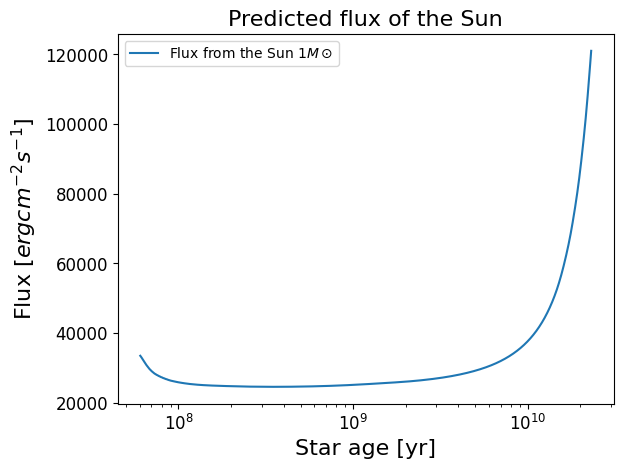
\includegraphics[width=\textwidth,height=0.5\textheight]{assets/fluxsun.png}
		\caption{Prediction for Flux of Sun $1 M\odot$.}
	\end{subfigure}
	\begin{subfigure}{\textwidth}
		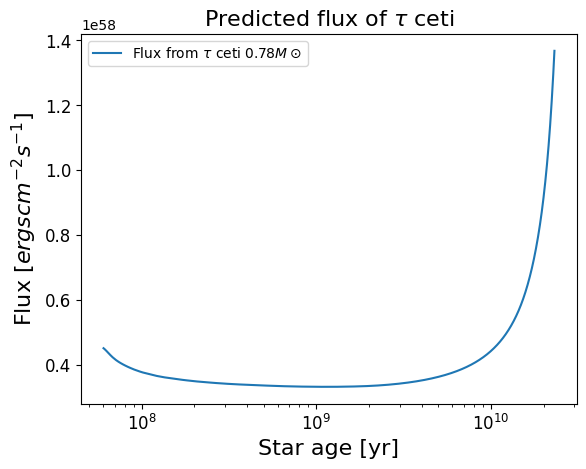
\includegraphics[width=\textwidth,height=0.5\textheight]{assets/fluxtau.png}
		\caption{Prediction for flux of $\tau$ ceti $0.78 M\odot$.}
	\end{subfigure}
	\label{fig:predicted flux}
\end{figure}

\clearpage
\section{Conclusion}

\clearpage

\titlecontents{section}[0pt]{\vspace*{1cm}}{}{}{\titlerule*[9pt]{.}\contentspage}

\singlespacing
\setlength{\bibitemsep}{\baselineskip}
\phantomsection
\bibliographystyle{apacite}
\bibliography{ref.bib}
\clearpage

\stopcontents[default]
\resumecontents[appendix]
\appendix
\titleformat{\section}[hang]{\center\bfseries\MakeUppercase}{APPENDIX \thesection: }{0pt}{}
\titlecontents{section}[0pt]{}{Appendix \thecontentslabel: }{}{\titlerule*[9pt]{.}\contentspage}

\section{Appendices}

\subsection{Data}

\begin{figure}[H]
	\centering
	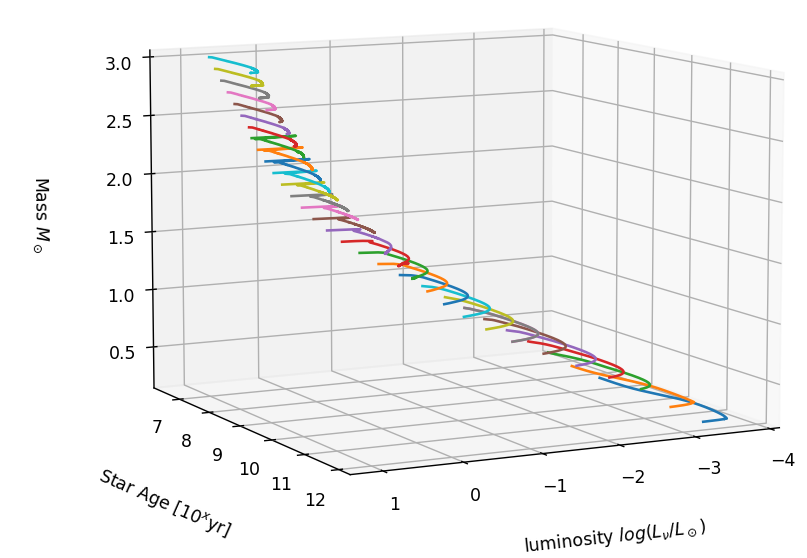
\includegraphics[width=\textwidth]{assets/3dpltdata.png}
	\caption{3D plot of Data for $0.2-3.0M_\odot$(only H burning).}
	\label{fig:3dplt}
\end{figure}
\begin{figure}[H]
	\centering
	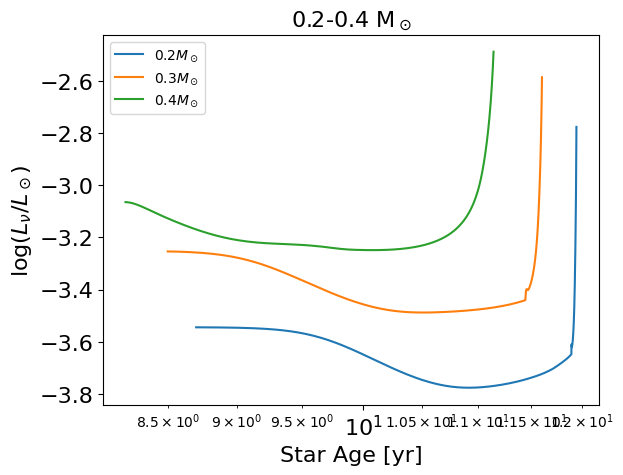
\includegraphics[width=\textwidth]{assets/Data0.2-0.4.png}
	\caption{Data for $0.2-0.5M_\odot$(only H burning).}
	\label{fig:0.2-0.4}
\end{figure}
\begin{figure}[H]
	\centering
	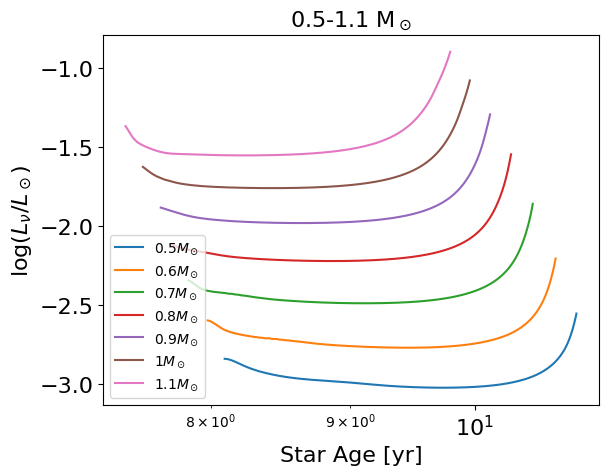
\includegraphics[width=\textwidth]{assets/Data0.5-1.1.png}
	\caption{Data for $0.5-1.1M_\odot$(only H burning).}
	\label{fig:0.5-1.1}
\end{figure}
\begin{figure}[H]
	\centering
	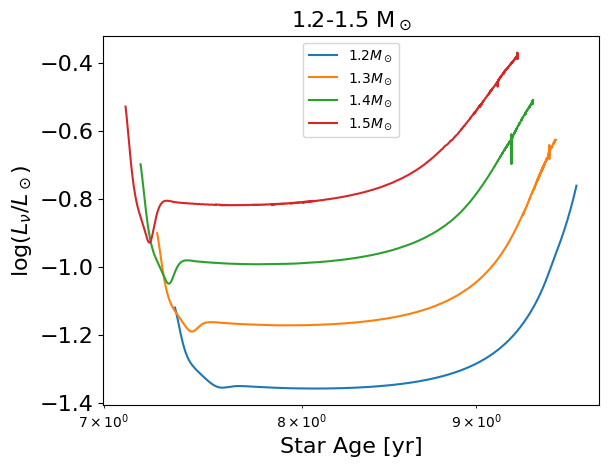
\includegraphics[width=\textwidth]{assets/Data1.2-1.5.png}
	\caption{Data for $1.2-1.5M_\odot$(only H burning).}
	\label{fig:1.2-1.5}
\end{figure}
\begin{figure}[H]
	\centering
	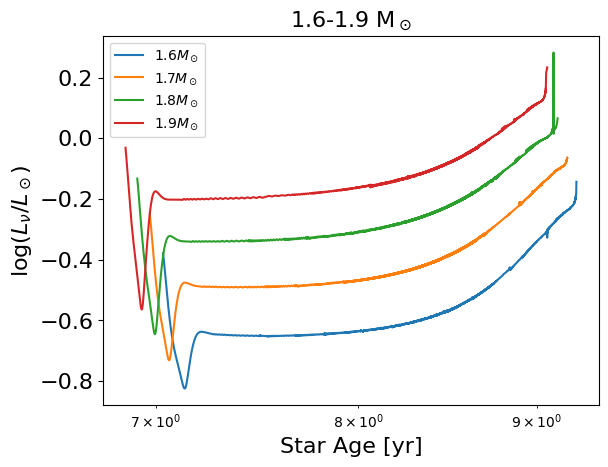
\includegraphics[width=\textwidth]{assets/Data1.6-1.9.png}
	\caption{Data for $1.6-1.9M_\odot$(only H burning).}
	\label{fig:1.6-1.9}
\end{figure}
\begin{figure}[H]
	\centering
	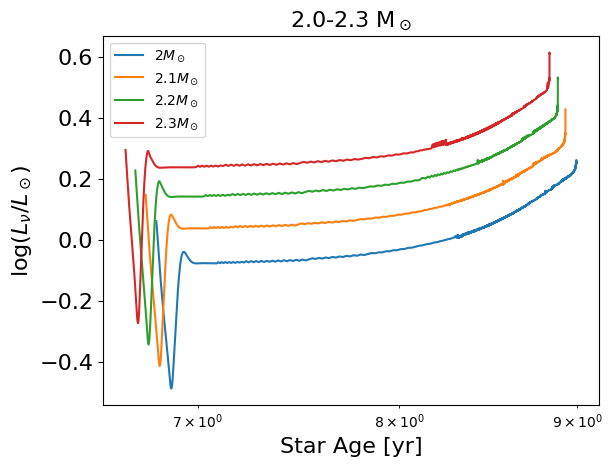
\includegraphics[width=\textwidth]{assets/Data2.0-2.3.png}
	\caption{Data for $2.0-2.3M_\odot$(only H burning).}
	\label{fig:2.0-2.3}
\end{figure}
\begin{figure}[H]
	\centering
	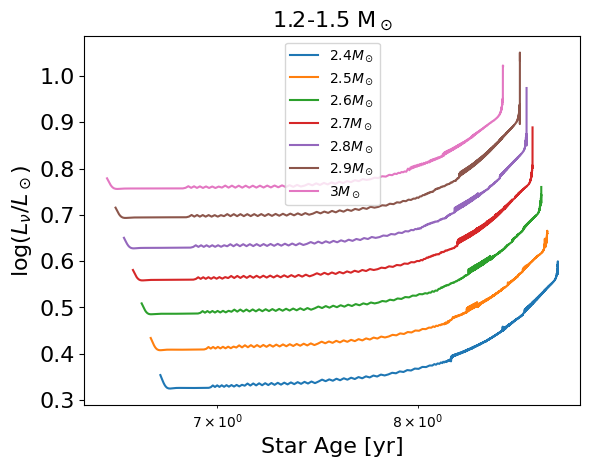
\includegraphics[width=\textwidth]{assets/Data2.4-3.0.png}
	\caption{Data for $2.4-3.0M_\odot$(only H burning).}
	\label{fig:2.4-3.0}
\end{figure}

\stopcontents[appendix]
\end{document}
